% !TEX root = ../my-thesis.tex
%
\chapter{Introduction}
\label{sec:intro}
\section{Background}
Controlling or even trying to prevent an infectious disease is a challenging task, and therefore it is crucial to find ways to combat this type of disease through new and creative ways. The number of infections can vary greatly between different countries or regions, and it is therefore of great interest for local governments or health institutes to find the underlying factors for these differences. This may lead to the identification of previously unrecognized environmental factors that could be the cause of the different risk of disease in different areas. One of the earliest examples of this type of analysis was carried out in relation to a cholera outbreak in south London in 1854 by John Snow. By creating the map shown in Figure~\ref{cholera}, he was able to show that cholera cases occurred mainly around a water pump in Broad Street. These findings were crucial to understanding that cholera spread through contaminated water supplies, and thus led to the modernization of water supply and sanitation systems in London and the rest of the world \autocite[][]{snow1857cholera}.
\begin{figure}[H]
    \centering
    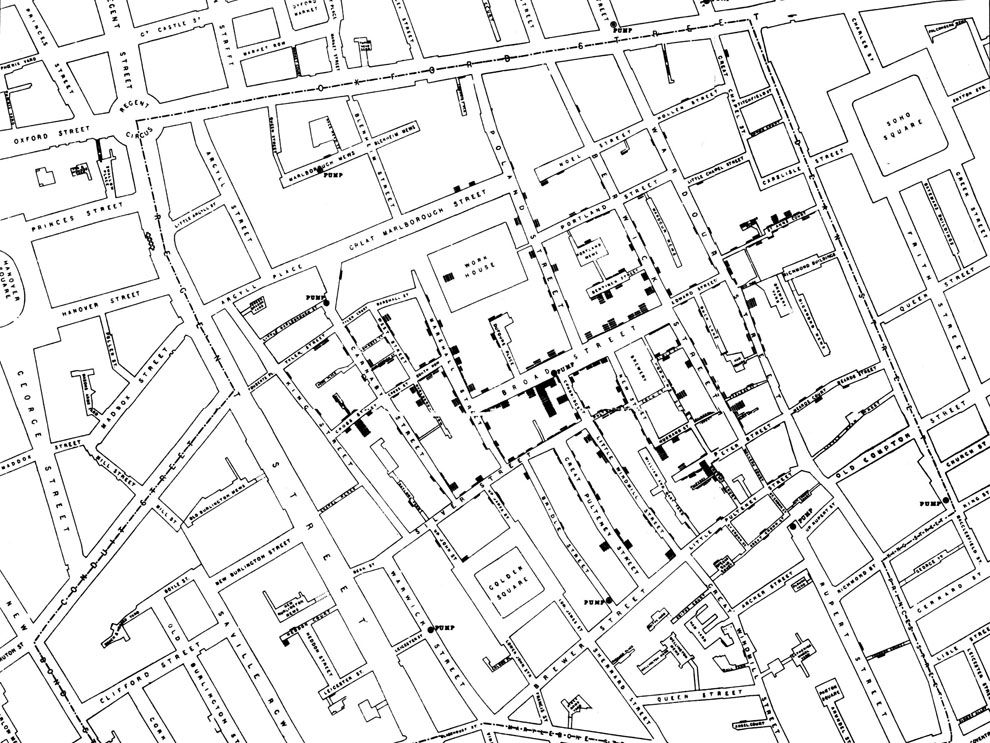
\includegraphics[width = 0.75\textwidth]{cholera_map.jpg}
    \caption{The original map of cholera cases in southern London, created by John Snow in 1854.}
    \label{cholera}
\end{figure}
The location itself (that is, a set of geographic coordinates) is generally unlikely to influence the risk of a certain disease; as there is no reason why one set of coordinates would inherently be at higher risk than another. Instead, the geographic location is a proxy measure, for differences in the attributes of the areas. These differences may relate to physical geography (e.g. temperature, sunlight, precipitation), environmental factors (e.g. air pollution, water quality) or population attributes (e.g. age, income, migration background). The identification of disparities in disease risk across a geographic region can lead to further investigation of the underlying reasons for the differences, which can lead to health breakthroughs such as those noted by Snow. Furthermore, by identifying areas of high risk, health authorities can focus additional resources on these areas in an attempt to influence the behaviours of the population that contribute to an increased risk of disease. \\
Most approaches to disease mapping are based on dividing the geographic region into spatial units, with disease risks estimated for each of these units. The reason for this is that individual-level data would violate patient confidentiality and governments are more interested in risk levels for the entire population. Each spatial unit has different demographics, so comparisons between spatial units are generally based on the standardized incidence ratio (SIR), defined as the number of observed cases in a given area divided by the number of cases expected for that area based on its population demographics.  Methodology for estimating disease risk can rely on conditional autoregressive (CAR) models \autocite[][]{besag1991bayesian}, which assume the existence of spatial autocorrelation between neighbouring areas, based on the notion that nearby areas are more likely to have more in common than areas that are further apart. This is due to the fact that adjacent areas are more likely to have similar socio-economic characteristics in terms of deprivation and population behaviour. It is assumed by these models that this level of spatial autocorrelation is constant across the spatial region.
\clearpage
\section{Corona Virus}
\label{sec:corona}
Viral diseases continue to pose a serious public health threat. Several viral epidemics have occurred in the last 20 years, including the Severe Acute Respiratory Syndrome (SARS) pandemic in 2002/3, H1N1 influenza in 2009, and more recently the Middle East Respiratory Syndrome Coronavirus (MERS-CoV), which was first detected in Saudi Arabia in 2012. \\
Cascella et al. provide a short summary of the key events of the outbreak as well as the characteristics of the disease, which is summed up in the remainder of this Section. \\
In late 2019, the first few cases of lower respiratory infections were detected in Wuhan, China. In February 2020, this viral disease was officially named "Covid-19", an acronym for "Coronavirus Disease 2019". \\
Due to the rapid spread of the virus, a Public Health Emergency of International Concern was declared at the end of January 2020, with 18 countries reporting cases and four countries reporting human-to-human transmission. \\
At the end of February 2020, the World Health Organization (WHO) raised the risk of a Covid-19 epidemic to "very high" before declaring it a pandemic on 11 March. At that time, more than 118,000 cases in 114 countries and 4000 deaths had already been registered. \\
The first cases of the disease were linked to direct exposure at the Huanan Seafood Wholesale Market in Wuhan, with animal-to-human transmission suspected as the main mechanism. After subsequent cases could not be linked to this mechanism, human-to-human transmission was presumed to be the main transmission mechanism. Furthermore, symptomatic individuals are thought to be the most common source of Covid-19 spread. However, asymptomatic individuals can transmit the virus, therefore isolation is the best way to contain this epidemic. \\
Similar to other respiratory diseases, e.g. influenza, transmission is thought to occur through respiratory droplets (particles $>5-10\mu m$ in diameter) when coughing and sneezing. In closed rooms, transmission by aerosol is possible. \\
Based on the data from the first cases in Wuhan, the incubation period is generally between 3 and 7 days, with a median of 5.1 days. According to the data, the number of infections doubled about every seven days and the basic reproductive number $R$ is 2.2, which means that on average each infected individual infects another 2.2 individuals. \\
According to a report by the Chinese Centre for Disease Control, which studied 72,314 cases, the overall mortality rate of confirmed cases was 2.3\%, with most of the fatal cases affecting people over 70 years of age. \\
Furthermore, the clinical manifestations of the disease can be divided into three groups according to their severity:
\begin{itemize}
    \item Mild disease: non-pneumonia and mild pneumonia; this occurred in 81\% of cases.
    \item Severe disease: dyspnea, respiratory rate $\geq 30$ min, blood oxygen level $\leq 93\%$; this occurred in 14\% of cases.
    \item Critical disease: respiratory failure, septic shock and/or multiple organ dysfunction or failure; this occurred in 5\% of cases.
\end{itemize}
Subsequent reports indicate that the disease is asymptomatic or with very mild symptoms in 70\% of patients, while the remaining 30\% develop a respiratory syndrome with high fever, cough and even severe respiratory failure, which may require admission to the intensive care unit. \\
Most countries use some kind of clinical and epidemiological information to determine who should be tested. A molecular test, for example a PCR test, can be used to detect the disease.\\
The WHO recommends the collection of samples from both the upper and lower respiratory tract. In the laboratory, the genetic material extracted from the saliva or mucus sample is amplified by reverse polymerase chain reaction (RT-PCR), which synthesizes a double-stranded DNA molecule from an RNA form. Once the genetic material is sufficient, the parts of the genetic code of the CoV that are conserved are searched for. The probes used are based on the original gene sequence published by the Shanghai Public Health Clinical Center \& School of Public Health, Fudan University, Shanghai, China on Virological.org and subsequent confirmatory evaluation by other laboratories \cite{cascella2021features}.
\clearpage
\section{Motivation}
Covid-19 has had a significant impact on the lives of almost everyone on Earth. Whether people had to work from home, children suddenly had online classes or people just stayed at home more, everyone was affected. Everyone had to adjust to this new reality where suddenly you could not meet for a coffee or go to the cinema together because those establishments were either closed or people had no desire to risk contracting Covid-19. And that, of course, says nothing about the impact it had on the lives of people who became infected with Covid-19, those who have had relatives who became infected and the more than 3 million people who have died as a result of the disease. The point is that everyone was affected by the impact of the pandemic, and still is, albeit at different levels. \\
Over time, different countries introduced different strategies to combat Covid-19, such as hard lockdowns where people were only allowed to leave the house if they had a legitimate reason to do so, for example to go to work or to buy groceries, while other countries did not introduce any lockdown measures. Other measures included wearing face masks in public places or limiting how many people can meet in public and private spaces. But even when the same measures were implemented in one country, there were big differences between the proportion of infected people in different parts of the country. \\
Finally, attitudes towards these measures have become a matter of political identity in various countries, as political parties from different spectrums have different views on how this pandemic should be handled, what measures should be implemented, or whether this pandemic even exists or if it is just much ado about nothing. This has led to the formation of new political movements that regularly protest against the measures taken by the government and demand a return to pre-pandemic conditions. \\
Understanding the reason why the number of infections varies in different parts of the country can be crucial in helping local governments decide which measures to implement to limit the risk of infection and contribute to the common goal of ending the pandemic as soon as possible. \\
Identifying areas where people are at higher risk of becoming infected can help governments decide on vaccination strategies, as it may make more sense to vaccinate people in high-risk areas first. By limiting the number of infections in these areas, the likelihood of the virus spreading from one of these areas to one or more neighbouring areas decreases, which in turn slows the spread of Covid-19.
\clearpage
\section{Aim and Objective}
The main goal of this work is to analyse what factors drive Covid-19 infection numbers and thus increase the risk of people becoming infected and getting sick from the virus. To identify these factors, it is possible to either look at current infection numbers across different areas to try to find patterns in the data, or to look at infection numbers across a spectrum of time and see if the likelihood of becoming infected changes when new factors, such as vaccination, are introduced or factors, such as government policies, change. Typically, Bayesian spatial models are used for disease mapping, where the neighbourhood structure between the areas of interest plays a crucial role. However, it is possible to neglect this structure and use a non-Bayesian approach to extract key factors. It is not possible to say that one class of models is superior to the other, as this depends mainly on the given data. Nevertheless, one of the aims of this work is to analyse infection counts from a non-temporal point of view and to compare the usefulness of a Bayesian spatial model with that of a non-Bayesian machine learning model. The other main objective of this work is to model the relationship between different features and infection numbers over a period of time using a temporal Bayesian model to see if any pattern emerges or identify which key factors have led to increased or decreased numbers of infections. \\
To answer these questions, a basic concept of Bayesian theory and Bayesian spatial models is developed and an introduction to geospatial data and the analysis of this particular type of data is given. In addition, a brief introduction to common machine learning methods is given. \\
For the analysis, different types of data need to be collected from different sources. For non-temporal modelling, these data include:
\begin{itemize}
    \item Data related to the number of infections in a given municipality.
    \item Data related to the number of vaccinations in a given municipality.
    \item Demographic data related to a specific municipality.
    \item Data related to spatial points of interest in a given municipality.
    \item Shapefiles for the geographic areas of interest.
\end{itemize}
For the temporal models, the following data is needed:
\begin{itemize}
    \item Data related to the number of infections in a given country
    \item Data related to the number of vaccinations in a given country
    \item Demographic data related to a given country
    \item Mobility trends in a given country
    \item Data keeping track of government measures in a given country
    \item Data on the relative frequency of different strains of Covid-19 in a given country.
\end{itemize}
In the analysis, these data are collected for two countries, Germany and Norway. These two countries are not equally affected by the pandemic and the population is distributed differently in the two countries, which makes for an interesting comparison of what factors influence the infection numbers and what kind of models work well in each country.\\
In order to achieve the main objectives of this thesis, the following important goals can be listed:
\begin{itemize}
    \item[1.] Build a basic concept of Bayesian theory, the analysis of geospatial health data as well as non-Bayesian machine learning models.
    \item[2.] Collect all the data needed for the analysis.
    \begin{itemize}
    \item[2.1] Collect data related to Covid-19 from the National Institutes of Health.
    \item[2.2] Collect demographic data and shapefiles from other official sources.
    \item[2.3] Collect infrastructure data by querying OpenStreetMap.
    \item[2.4] Collect data for mobility trends and government measures from Our World in Data (OWID).
    \item[2.5] Collect data on the frequency of Covid-19 strains from the open-source project CoVariants.
    \end{itemize}
    \item[3.] Merge all data from different sources to create clean datasets for the analysis.
    \item[4.] Develop and compare different types of Bayesian spatial models.
    \item[5.] Train non-Bayesian machine learning models and compare them to the Bayesian models.
    \item[6.] Develop and compare different types of Bayesian temporal models.
    \item[7.] Critically evaluate the models and extract factors that significantly influence the risk of infection.
\end{itemize}
\clearpage
\section{Related Work and Contribution}
Since the start of the pandemic in 2019, numerous scientific papers have been written on Covid-19, covering a wide range of topics within medicine, social sciences and statistics. Some papers have been written on the relationship between geographic regions and Covid-19. Incorporating a spatial dimension into the research process can help to better understand different phenomena and make them potentially mappable. The papers considered here can be divided into two categories. The first group consists of disease mapping, spatial analysis and spatio-temporal analysis and refers to studies that analyse the spatial and spatio-temporal patterns of Covid-19. The other group contains research that focuses on other factors that influence the dynamics of the Covid-19 pandemic, but may include spatial and spatio-temporal analysis.
\subsection{Disease Mapping, Spatial Analysis and Spatio-Temporal Analysis}
\cite{guan2020clinical}, study cases in mainland China up to 25 February 2020 to determine the defining clinical features and severity of the disease. Among others, they find that Covid-19 spread rapidly through the country and that the severity of the disease varied. Furthermore, they find that the most common symptoms experienced by patients are cough and fever. They report a median incubation period of 4 days.\\
\cite{chen2020distribution} analyse how people who emigrated from Wuhan contributed to the early stages of the pandemic in China at the beginning of 2020. They find a strong correlation between the number of confirmed cases of Covid-19 in a given province and emigration from Wuhan. They find that the lockdown of several cities in Hubei province and the implementation of nationwide control measures were effective in preventing the exponential growth of the number of cases. \\
Similar to this study, \cite{gross2020spatio} compare the infection rate in different cities in China and provinces in Italy during the early phases of the pandemic and conclude that the spread of the disease is defined by a two-stage process. The first stage, the authors say, is defined by a constant rate of infection due to a lack of means to detect infected individuals before symptoms appear. In the second stage, they observe an approximately exponential decline due to quarantine. While they find differences between China and Italy, most notably that it took longer for outbreaks of the disease to be controlled in the Italian provinces, they find similar behaviour in terms of infection rate. \\
\cite{chen2021spatio} analyse the spatio-temporal distribution characteristics and influencing factors of the virus in mainland China using statistical methods, correlation analyses and geographic information system (GIS) mapping. They conclude that the outbreak in non-Hubei provinces can be divided into five phases. The initial outbreak phase, the peak phase where the highest number of new infections is observed, the containment phase where the number of new infections decreases, the rebound phase and a final phase where the number of new infections flattens out. They observe that cities with large population flows from Wuhan were more affected by Covid-19. \\
\cite{saha2020monitoring} provide an overview of how GIS, e.g. mapping dashboards and applications, can be used to monitor the pandemic and related activities. They conclude that the pandemic requires massive data generation and GIS to enable rapid response and analysis to help prevent and guide decisions and movements. \\
\cite{gianquintieri2020mapping} use geo-referenced calls to the emergency number relevant to respiratory problems and subsequent emergency medical service interventions to derive an unbiased representation of Covid-19 diffusion. This study is conducted for the Lombardy region of Italy, which was particularly hard hit by the pandemic in early 2020. The authors report a strong correlation between Covid-19-related deaths at the provincial level and emergency calls and age- and sex-weighted ambulance dispatches.\\
Lastly, \cite{petrov2020spatiotemporal} examine the spatio-temporal dynamics of the pandemic in the Arctic up to July 2020. They find that the number of infections and morbidity are highly variable, but generally below national levels. They classify the Arctic regions into four groups: Iceland, the Faroe Islands, northern Norway and northern Finland, which are characterized by increased early infection rates but containment of the pandemic through quarantine and other measures; Northern Sweden and Alaska, where the first wave of infection persisted despite weak (Sweden) or variable (Alaska) quarantine measures; northern Russia, where a late start led to a steep rise in infections, deaths and several outbreaks; and northern Canada and Greenland where there was no significant spread of the pandemic.
\subsection{Other Factors Influencing the Pandemic}
\cite{xiong2020spatial} carry out a correlation analysis for the number of cases in the Hubei province between 30 January 2020 and 18 February 2020. They find a significant correlation between population, regional GDP, retail sales of consumer goods and the number of confirmed cases of Covid-19 in Hubei province, among others. \\
\cite{ahmadi2020investigation} analyse the influence of climatic factors on the spread of Covid-19 in Iran and find that areas with low wind speed, humidity and solar radiation support the survival of the virus. The same study finds a direct correlation between population density and movement within provinces. \cite{mehmood2021spatiotemporal} analyse the relationship between air pollution, climate, socioeconomic factors and infection rates in Pakistan. They report a significant positive correlation between particulate matter $\left(\hbox{PM}_{2.5}\right)$, an air pollutant, and the number of infections. In contrast to Ahmadi et al., the correlation between the factors humidity and wind speed and the number of infections is positive in some regions and negative in others. They find a small negative relationship between population density and Covid-19 cases, suggesting that areas with higher population density reported proportionally fewer cases.\\
\cite{pedrosa2020dynamics} analyses the relationship between the number of cases in the US and weather, demographic variables and the infection timeline. He finds that only population density and a time series variable, defined as the number of days between the first and the 100th case, showed statistical significance, while the climate in the USA has no influence on infection numbers.\\
As the United States is one of the countries most affected by the pandemic, many studies have attempted to determine what factors are driving up the number of infections in the country. \cite{mollalo2020gis} analyse the spatial variability of Covid-19 in the United States up to the 9 April 2020. Out of 35 environmental, socio-economic, topographical and demographic variables, the four variables found to be most significant were: income inequality, median household income, the proportion of black females and the proportion of nurse practitioners at the county level. \\
\cite{maiti2021exploring} analyse infection counts up to 13 May 2020 in the USA. They observe a higher risk of Covid-19 clusters in metropolitan areas compared to rural counties, counties near central airports, more populous counties and counties with the highest proportion of racial and ethnic minorities. \\
\cite{wang2021spatiotemporal} analyse the numbers up to 29 January 2021 in the US and find that factors of ethnicity, crime and income have positive correlations with the number of Covid-19 cases and explain most of the variance in the modelling estimate. \\
\cite{allcott2020polarization} examine partisan differences in Americans' responses to the Covid-19 pandemic, specifically how Republicans and Democrats socially distance themselves and make other efforts to reduce transmission of the disease. They model not the risk of being infected, but how a person's political beliefs affect their beliefs about the Covid-19 pandemic. They find significant individual-level differences between Republicans and Democrats in self-reported social distancing, beliefs about their personal risk of being infected, and beliefs about the future severity of the pandemic. According to the study, Democrats find it significantly more important to stay inside to prevent the spread of the virus than to go outside to help the economy, compared to Republicans. \\
\cite{bermudi2021spatiotemporal} model mortality in the country using latent Gaussian-Bayesian spatial models and find significant relationships between Covid-19 mortality and socioeconomic conditions, as higher socioeconomic levels, as measured by a socioeconomic index, are shown to lead to a lower risk of mortality due to Covid-19. In addition, they show that men and older persons had the highest risk of mortality due to Covid-19. \cite{castro2021spatiotemporal}, on the other hand, could not find a single narrative that explains the spread of the virus across the states of Brazil, but rather find that layers of complex scenarios intertwine, resulting in a different and simultaneous Covid-19 epidemic across Brazil. \\
The situation in India is analysed in a paper by \cite{nandy2021managing} and the authors find that higher investment in health and education reduces the likelihood of the spread of Covid-19. In addition, a higher cure rate is found in states with sustained investment in health and education, with mortality rates lower in states that invest more in education. \\
\cite{sannigrahi2020examining} find a significant correlation between selected demographic and socio-economic components, including total population, poverty and income, and the number of deaths from Covid-19 in Europe, without controlling for other factors such as environmental variables, socio-ecological status or climate extremes. \\
Studies have been conducted analysing the impact of interdiction measures on the spread of Covid-19. \cite{kasilingam2020exploring} attempt to predict early containment of Covid-19 using machine learning models based on infrastructural and environmental variables, as well as government-implemented policies and infection-related independent variables for 42 countries. Using logistic regression, a significant positive association is found between healthcare infrastructure and lockdown policies and signs of early containment. 
\cite{orea2020effective} find a significant positive relationship between interdiction in Spain and its usefulness in preventing the spread of Covid-19 between different provinces in Spain. Furthermore, the same type of relationship is found for the spread of Covid-19 within the same province. \\
\subsection{Contribution}
The information contained in all the papers mentioned earlier shows just how many factors may or may not be associated with the way that Covid-19 spreads in different countries. Finding a perfect model that explains why numbers are higher in one geographical region than in another is utopian, as there are still too many unknowns even more than a year into the pandemic. Achieving a scientific breakthrough is therefore beyond the scope of this work, the aim is rather to consider a wide range of factors, including infrastructural factors, demographic and socio-economic variables, when discussing the reason for different infection figures within a country and between two different countries. The countries selected for this work, Norway and Germany, are not equally affected by Covid-19, so looking for factors that influence infection numbers in both countries may be indicative of a variable that is driving infection numbers up or down, independent of the country. Of particular interest to this thesis is the link between the political views of people within a municipality and the infection rates in the municipality. Since Germany has been experiencing a lot of anti-hygiene demonstrations and a lot of criticism comes from the right side of the political spectrum, the decision was made to take a close look at whether there is a correlation between the share of votes that certain political parties receive in a given area and the number of infections in that area.
\clearpage
\section{Thesis Outline}
The structure of the thesis is as follows. First, an introduction to Bayesian inference is given in Chapter~\ref{sec:bayes}. This part includes basic concepts of Bayesian theory, e.g. Bayes' theorem, which are essential for the methodology used in this thesis. Furthermore, different types of priors are introduced, as they form an integral part in Bayesian modelling. In addition, Markov-chain-Monte-Carlo-methods (MCMC methods), latent Gaussian models and Integrated Nested Laplace Approximation are introduced, the latter of which can overcome the shortcomings of MCMC methods and form the basis for Bayesian spatial models. The last part of this chapter includes the introduction of goodness-of-fit indicators used to evaluate model performance and addresses some problems of Bayesian spatial models. \\
In Chapter~\ref{sec:geodata} a brief introduction to the analysis of geospatial health data is given. First, different types of geospatial data, namely vector data and raster data, are introduced before discussing different methodologies used in modelling this type of data. These methodologies include the standardized incidence ratio (SIR) and the estimation of disease risk in spatial areas. \\
A short introduction to machine learning is given in Chapter~\ref{ch:ml}. Several commonly used machine learning algorithms are introduced in Section~\ref{sec:algo} before providing a short review of machine learning methodology and introducing a recent field in machine learning, interpretable machine learning, in Section~\ref{sec:methods}. \\
Chapter~\ref{sec:datacollection} gives a brief overview of the different types of data collected in this thesis and how the different data sources were combined into a coherent dataset. 
Chapter~\ref{sec:analysis} focuses on the analysis of this data. First the SIR for the countries is examined, followed by the modelling of the relationship between variables of interest and the infection numbers in Norway and Germany. First, a Bayesian approach to this problem is shown, consisting of models that do not take the neighbourhood structure in the respective countries into account and models that do take such a structure into account. Section~\ref{sec:hyperprios} analyses how these models change, when the prior distribution that is used in the modelling process is changed. Next, non-Bayesian models that are built using the methodology introduced in Section~\ref{sec:algo} are discussed and compared to the Bayesian models. Finally, Bayesian temporal models are evaluated in Section~\ref{sec:temporal}. \\
As part of this thesis, a dashboard that gives an overview over the used data and allows the modelling of spatial and temporal relationship was developed. A summary of the functionality of this dashboard is find in Chapter~\ref{ch:shiny}.
The relevant findings of the models calculated during the analysis are discussed in Chapter~\ref{sec:discussion} before the research is wrapped up in Chapter~\ref{sec:conclussion}, summing up the most important insights of this thesis.